\documentclass[12pt]{article}
\usepackage[top=1in, bottom=1in, left=1in, right=1in]{geometry}

\usepackage{setspace}
\onehalfspacing

\usepackage{amssymb}
%% The amsthm package provides extended theorem environments
\usepackage{amsthm}
\usepackage{epsfig}
\usepackage{times}
\renewcommand{\ttdefault}{cmtt}
\usepackage{amsmath}
\usepackage{graphicx} % for graphics files
\usepackage{tabu}

% Draw figures yourself
\usepackage{tikz} 

% writing elements
%\usepackage{mhchem}

\usepackage{paralist}

% The float package HAS to load before hyperref
\usepackage{float} % for psuedocode formatting
\usepackage{xspace}

% from Denovo Methods Manual
\usepackage{mathrsfs}
\usepackage[mathcal]{euscript}
\usepackage{color}
\usepackage{array}

\usepackage[pdftex]{hyperref}
\usepackage[parfill]{parskip}

% math syntax
\newcommand{\nth}{n\ensuremath{^{\text{th}}} }
\newcommand{\ve}[1]{\ensuremath{\mathbf{#1}}}
\newcommand{\Macro}{\ensuremath{\Sigma}}
\newcommand{\rvec}{\ensuremath{\vec{r}}}
\newcommand{\vecr}{\ensuremath{\vec{r}}}
\newcommand{\omvec}{\ensuremath{\hat{\Omega}}}
\newcommand{\vOmega}{\ensuremath{\hat{\Omega}}}
\newcommand{\even}{\ensuremath{\phi^g}}
\newcommand{\odd}{\ensuremath{\vartheta^g}}
\newcommand{\evenp}{\ensuremath{\phi^{g'}}}
\newcommand{\oddp}{\ensuremath{\vartheta^{g'}}}
\newcommand{\Sn}{\ensuremath{S_N} }
\newcommand{\Ye}[2]{\ensuremath{Y^e_{#1}(\vOmega_#2)}}
\newcommand{\Yo}[2]{\ensuremath{Y^o_{#1}(\vOmega_#2)}}
\newcommand{\sigg}[1]{\ensuremath{\Macro^{gg'}_{s\,#1}}}
\newcommand{\psig}{\ensuremath{\psi^g}}
\newcommand{\Di}{\ensuremath{\Delta_i}}
\newcommand{\Dj}{\ensuremath{\Delta_j}}
\newcommand{\Dk}{\ensuremath{\Delta_k}}
%---------------------------------------------------------------------------
%---------------------------------------------------------------------------
\begin{document}
\begin{center}
{\bf NE 255, Fa16 \\
Acceleration and Preconditioning\\
November 1, 2016}
\end{center}

\setlength{\unitlength}{1in}
\begin{picture}(6,.1) 
\put(0,0) {\line(1,0){6.25}}         
\end{picture}

We've talked about basic methods for inner, outer, and eigenvalue iterations. We've talked a bit about how and why some methods are faster than others as well as when some methods might struggle with converging quickly. We're next going to talk about the fundamental idea of preconditioning and acceleration methods. We'll then go into methods specifically used in Nuclear Engineering. 

First recall that \underline{conditioning} is one way to express the perturbation behavior of the mathematical problem. A \emph{well-conditioned} problem is one in which all small perturbations of $x$ lead to only small changes in $f(x)$. An \emph{ill-conditioned} problem is one in which some small perturbation of $x$ leads to a large change in $f(x)$. The condition number is a quantity used to express how well-conditioned a matrix or problem is. A small condition number corresponds to a well-conditioned problem, and vice versa. 

The condition number of an $n \times m$ matrix $\mathbf{A}$ is defined as
%
\begin{equation}
  \kappa(\mathbf{A}) = ||\mathbf{A}|| \text{ }||\mathbf{A}^{-1}|| = \frac{\sigma_{1}}{\sigma_{m}}\:,
  \label{eq:condA}
\end{equation}
%
where $\sigma_{1} \ge \sigma_{2} \ge \dots \ge \sigma_{n} > 0$ are the singular values of $\ve{A}$. If $\mathbf{A}$ is singular, its condition number is infinity. 

A way to think about the condition number: the ratio $\frac{\sigma_{1}}{\sigma_{m}}$ can be interpreted as the eccentricity of the hyper-ellipse that is the image of an $m$-dimensional unit sphere under $\mathbf{A}$. When $\ve{A}$ has a large condition number the largest principle semiaxis is much longer than the smallest principle semiaxis. 

(again, taken from my dissertation)

\subsection*{Preconditioning}
The new ``grand challenge'' problems facing the nuclear transport community are large and complex. Cutting edge methods are required to solve them. While we've discussed methods that enable the solution of such problems, low-cost preconditioners that can reduce the number of iterations needed for convergence will be invaluable. This is true for Krylov methods in particular because the memory required and cost per iteration increase dramatically with the number of iterations. %\cite{Benzi2002}. And, as discussed in Chapter \ref{sec:Chp3}, 
Krylov methods can converge very slowly for poorly conditioned systems. 

The general idea of preconditioning is to transform the system of interest into another equivalent system that has more favorable properties, for example one with a smaller condition number. A preconditioner is a matrix that induces such a transformation by improving the spectral properties of the problem being solved. Let $\ve{G}$ be a non-singular preconditioner, then $\ve{A}x=b$ can be transformed in the following ways:% \cite{Benzi2002}: 
%
\begin{alignat}{3}
  \ve{G}^{-1}\ve{A}x &= \ve{G}^{-1}b  &  &\text{left preconditioning,} \\
  \ve{AG}^{-1}y &= b, \qquad  &x = \ve{G}^{-1}y \qquad &\text{right preconditioning, and } \\
  \ve{G}_{1}^{-1}\ve{AG}_{2}^{-1}y &= \ve{G}_{1}^{-1}b, \qquad \ve{G} = \ve{G}_{1}\ve{G}_{2}, \qquad  &x = \ve{G}_{2}^{-1}y  \qquad &\text{split preconditioning.} 
\end{alignat}

If $\ve{A}$ and/or $\ve{G}$ are non-normal then each of the preconditioning constructs will likely give different behavior, though they will converge to the same answer because the matrices are similar and therefore have the same eigenvalues. %\cite{Benzi2002}. 
Right preconditioning leaves the right hand side of the equation unaffected and does not change the norm of the residual, which is used for convergence testing in most iterative methods. Right preconditioning is usually preferred over left preconditioning for iterative solvers for this reason. %\cite{Knoll2004}. 
The remaining discussion will be presented in right preconditioner format. 

The matrix $\ve{A}\ve{G}^{-1}$ is typically not formed in practice. The preconditioner can be applied by using some method to solve $\ve{G}y=c \to y \approx \ve{G}^{-1}c$, or by otherwise implementing the action of $\ve{G}^{-1}$ without ever explicitly forming and inverting $\ve{G}$. There are two extremes between which all other preconditioners lie: $\ve{G} = \ve{A}$, in which case the solution can be found directly, and $\ve{G} = \ve{I}$, which will have no effect.% \cite{Benzi2002}, \cite{Trefethen1997}. 

Functionally, a good preconditioner should make the system easier to solve and result in faster convergence. It should also be cheap to construct and apply. These tend to be competing goals in that the easier a preconditioner is to construct and apply the less it typically does to improve convergence. A preconditioner is considered good if $\ve{A}\ve{G}^{-1}$ is not too far from normal and its singular values are clustered.% \cite{Trefethen1997}. 

There are many different types of preconditioners, but they can be put into two general categories: \textbf{matrix-based} and \textbf{physics-based}. Matrix-based preconditioners rely entirely on the structure of the matrix $\ve{A}$ regardless of the physics of the problem. That is, these methods do not change when the underlying problem changes. This can be a very useful property because matrix-based methods are then broadly applicable and do not require any understanding of the physical problem. Extrapolation methods and incomplete factorizations are examples of matrix-based preconditioners.% \cite{Trefethen1997}.

Physics-based preconditioning uses knowledge about the physics of the problem in question to guide the creation of the preconditioner. This means that some methods only work with certain kinds of problems, and that the preconditioners may have to be tailored or adapted for different applications. However, such methods take advantage of knowing something about the problem and can be more effective than matrix-based methods for the range of problems for which they are intended. Rebalance and synthetic acceleration are examples of physics-based preconditioners.% \cite{Trefethen1997}.


\subsubsection*{Extrapolation Methods}
Extrapolation methods were historically used to accelerate $k$-eigenvalue calculations. These tend to be based on simple iterative solvers or polynomial approximations. One step of a simple iterative method such as Jacobi, Gauss Seidel, or successive over relaxation (SOR) can be used at the outset of a problem to serve as a preconditioner. %\cite{Trefethen1997}. 
When applied to neutron transport, an overrelaxation method looks like $\ve{F}_{i+1} = \omega(\tilde{\ve{F}}_i - \ve{F}_i) + \ve{F}_i$ with $1 \le \omega < 2$, where the unaccelerated new iterate for the fission source is designated $\tilde{\ve{F}}_i$.% \cite{Lewis1993}.

Polynomial preconditioners create a matrix polynomial $\ve{G}^{-1} = p(\ve{A})$, where $p(\ve{A})$ serves as a polynomial approximation to $\ve{A}^{-1}$. Common polynomial choices are truncated Neumann series and Chebyshev polynomials. An advanced variation of this method is to determine the polynomial coefficients adaptively. %\cite{Trefethen1997}. 
When Chebyshev polynomials are applied to the transport equation, $\ve{F}_{i+1} = \ve{F}_i + \alpha_{i+1}(\tilde{\ve{F}}_i - \ve{F}_i) + \beta_i(\ve{F}_i - \ve{F}_{i-1})$, where $\alpha$ and $\beta$ are iteration dependent. %\cite{Lewis1993}. 
Neither of these extrapolation methods are widely used today as they have not been very successful in multi-dimensional problems. There are analogous versions of these methods for fixed source problems.% \cite{Alcouffe1977}.  

\subsubsection*{Rebalance}
Rebalance methods are designed to accelerate iteration on the scattering or fission source by imposing a balance condition on the unconverged solution over either coarse or fine regions. If the region is coarse, this is a coarse-grid approximation preconditioner since fine-grid physics are excluded. If the region is fine, this is a local approximation preconditioner where short range effects are permitted and long range interactions are excluded.% \cite{Trefethen1997}, \cite{Adams2002}.

In either case, the unaccelerated solution is multiplied by a constant in each region that satisfies the balance equation. The rebalance process adjusts the average amplitude of the flux over a region and the iteration adjusts the space-angle distribution. The notion is that these processes work in concert to eliminate all error modes simultaneously.% \cite{Adams2002}. 

Coarse mesh rebalance (CMR) has been more successful than the fine version and is therefore used more often. In practice, choosing regions properly must be done with care. %\cite{Lewis1993}. 
Traditional forms of CMR can be unstable for problems where the spatial mesh is large compared to the neutron mean-free-path and where the scattering ratio is close to unity.% \cite{Alcouffe1977}. 

\subsubsection*{Incomplete Factorizations}
%Incomplete factorization methods were first introduced in the 1950s by Buleev, and independently by Varga. In the late 1970s these methods started gaining popularity, and since then have been under active development. 
The idea is to partially factor the matrix $\ve{A}$ such that the resulting matrices are sparse enough to take advantage of sparse solver methods, but close enough to $\ve{A}$ to be valuable as preconditioners.% \cite{Benzi2002}.

Incomplete Cholesky (IC) or incomplete LU (ILU) factorization have both been extensively used within the nuclear community. The Cholesky version is used when $\ve{A}$ is symmetric and LU when non-symmetric. Factorizations typically destroy sparsity, resulting in matrices that are denser than the originals and making their use more costly. Different variations of incomplete factorization methods address this by permitting the new matrices to have values only in positions where $\ve{A}$ has values, allowing a prescribed amount of fill in, or only saving entries greater than some tolerance.% \cite{Trefethen1997}, \cite{Patton2002}, \cite{Oliveira1998}.

\subsubsection*{Synthetic Acceleration}
In synthetic acceleration a low-order approximation to the transport operator is used to accelerate the full transport problem. %\cite{Lewis1993}. 
If a system is discretized with a high-order method it can be preconditioned with a lower-order approximation. The low-order method is often much sparser than the original, but still captures the general behavior of the problem. %\cite{Trefethen1997}. 
This is generally done with either the diffusion equation, giving diffusion synthetic acceleration (DSA), or a transport equation that is simpler than the one actually being solved, giving transport synthetic acceleration (TSA). These can be used for fission or fixed source problems.% \cite{Adams2002}. 

Synthetic methods have at least two iteration stages. The simplest way to illustrate this is to use source iteration for the within-group solver. The first step is a transport sweep, giving:
%
\begin{equation}
  \ve{L}\psi^{(l+\frac{1}{2})} = \ve{S}\psi^{(l)} + q \:, \qquad l \ge 0 \:.
  \label{eq:synthetic}
\end{equation}
%
Here $l$ is the iteration index, $\ve{L}$ is the transport operator, $\ve{S}$ is the scattering matrix, and $q$ is the external source. Equation \eqref{eq:synthetic} is subtracted from the exact equation to get an expression for an exact additive correction:
%
\begin{equation}
  \bigl( \ve{L} - \ve{S} \bigr)\bigl( \psi - \psi^{(l+\frac{1}{2})} \bigr) = \ve{S}\bigl(\psi^{(l+\frac{1}{2})} - \psi^{(l)} \bigr) \:.
  \label{eq:correction}
\end{equation}
%
This cannot be solved exactly, but the idea of synthetic methods is to find an $\ve{G}^{-1} \approx (\ve{L} - \ve{S})^{-1}$ that will be easier to evaluate than $(\ve{L} - \ve{S})^{-1}$. Equation \eqref{eq:synthetic} is solved by a high-order scheme and Equation \eqref{eq:correction} is solved with a low-order approximation. If the synthetic system converges, it must satisfy the original transport equation.% \cite{Adams2002}. 

Original DSA formulations exhibited instability in some instances. In 1977 Alcouffe demonstrated with diamond difference that stability can be obtained by using a consistent spatial differencing scheme. %\cite{Alcouffe1977}. 
The transport and diffusion equations cannot be discretized independently or the diffusion equation may not satisfy the original transport equation. The discretization of the diffusion equation must therefore be derived from the discretization of the transport equation such that they are consistent. Alcouffe's idea has since been extended to accelerate currents, to more dimensions, and to different spatial discretizations.% \cite{Larsen1982}. 

DSA can be implemented a few different ways, each of which performs a transport sweep and then solves a corrected diffusion equation. Different terms in the diffusion equation can be corrected for different problem types. %\cite{Alcouffe1977}. 
DSA has been found to degrade in the presence of material discontinuities in addition to when it is not consistently derived. However, Warsa et al.\ found that when DSA is used as a preconditioner for Krylov iterative methods, it is effective even when only partially consistent.% \cite{Warsa2004}.

To address the concerns about spatial discretization associated with DSA, a low-order transport solve could be used to find the correction term instead. Larsen and Miller developed a method that neglects scattering in the low-order transport equation, but this can cause instability in multi-dimensional problems. %\cite{Larsen1986}. 
Ramone et al.\ proposed including some scattering by using a tunable parameter. A high-order transport equation is solved first, then a transport equation with a coarse quadrature and reduced scattering is solved to find the correction that is applied to the new iterate of the scalar flux. %\cite{Ramone1997}. 
This algorithm can be viewed as Richardson iteration with a coarse operator preconditioner. Synthetic acceleration methods are widely used and actively researched in the transport community today. 

%-----------------------------------------------------------------------------------------------------
\subsubsection*{DSA in Transport}
DSA is typically used to precondition the within-group transport equation, $\bigl(\ve{I} - \ve{DL}^{-1}\ve{MS}_{gg}\bigr) \phi_{g} = \ve{DL}^{-1}Q_{g}$, which works very well when using a Krylov method. High-frequency error modes are what often cause instability in DSA. Krylov iteration, like iterative methods in general, will rapidly damp such oscillatory modes. Eliminating the high-frequency error enables the removal of the consistency requirement since DSA is not likely to fail when those error modes are gone. %\cite{Evans2009d}. 
This means DSA can be applied successfully for a variety of spatial discretizations. 

The DSA-preconditioned one-group equation is:
%
\begin{equation}
  \bigl(\ve{I} + \ve{PC}^{-1}\ve{RS}\bigr) \bigl(\ve{I} - \ve{DL}^{-1}\ve{MS}\bigr) \phi = \bigl(\ve{I} + \ve{PC}^{-1}\ve{RS}\bigr)\ve{DL}^{-1}\bar{Q} \:. 
  \label{DSA1group}
\end{equation}
%
Here $\ve{C}$ is the diffusion operator; %defined in Appendix~\ref{sec:AppendixA}; 
$\ve{R}$ is the restriction operator that maps the transport solution onto the diffusion vector; and $\ve{P}$ is the projection operator that maps the diffusion vector onto the transport solution. Most codes do not actually form these operators, instead they solve the diffusion equation and update the $\phi_{00}$ moments. In practice this means that for a Krylov iteration
%
\begin{equation}
  \ve{C}z = \ve{RS}\bigl(\ve{I} - \ve{DL}^{-1}\ve{SM}\bigr) v
\end{equation}
%
is solved for each group. DSA has been found to be beneficial for diffusive problems with high scattering ratios that are close to being isotropic. %\cite{Evans2009d}. 
%This is consistent with experiences of the wider nuclear community.


%-----------------------------------------------------------------------------------------------------
\subsection*{Multigrid Methods}
%The new preconditioner added to Denovo does multigrid in the energy dimension. To understand why multigrid in energy makes sense, why multigrid methods work must be understood. The material presented here is largely from \emph{A Multigrid Tutorial} by Briggs, Henson, and McCormick \cite{Briggs2000}, supplemented by Dr. Strang's lectures on multigrid and preconditioners available as MIT Open Courseware \cite{Strang}.
Multigrid methods take advantage of the fact that the error in any solution guess, $v$ for the system $\ve{A}u=b$, can be written as a combination of Fourier modes. [The algebraic error is given by $e = u - v$; since $e$ cannot be calculated exactly (otherwise the answer would be known), the residual $r = b - \ve{A}v$ is used instead.] A Fourier mode is described by a wavenumber, $k$, which denotes the frequency of oscillation. The $j$th Fourier mode is 
% 
\begin{equation}
    e_{j} = \sin\bigl(\frac{jk\pi}{n}\bigr) \:, \qquad 0 \le j \le n \:, \qquad 1 \le k \le n-1 \:.
\end{equation} 
%
There are $k$ half sine waves that comprise $e$ on the domain of the problem. The term $e_{k}$ indicates an $e$ with wavenumber $k$. The $k$th wave has $\frac{k}{2}$ full sine waves with a wavelength of $\frac{2}{k}$. Modes with wavenumbers in the range $1 \le k \le \frac{n}{2}$ are called low-frequency or smooth modes and those in $\frac{n}{2} \le k \le n-1$ are called high-frequency or oscillatory modes. Figure \ref{fig:FourierModes} shows what a few different modes look like. 
%
\begin{figure}[!ht]
    \begin{center}
      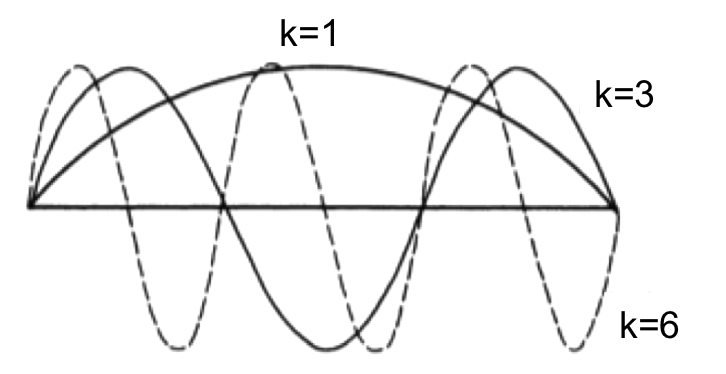
\includegraphics [width=0.45\textwidth, height=0.2\textheight] {fig/FourierModes}
   \end{center}
   \caption{Three Fourier Modes}% \cite{Briggs2000}}
   \label{fig:FourierModes}
\end{figure}

Iterative methods, also referred to as smoothers or relaxers, remove high frequency error components very quickly, but take a long time to remove the low frequency components. %This is illustrated in Figure~\ref{fig:FourierError}, where weighted Jacobi was applied to Fourier modes of different frequencies on an $n$ = 64 grid. The error is reduced much faster for higher modes. 
%
%\begin{figure}[!ht]
%    \begin{center}
%      \includegraphics [width=0.5\textwidth, height=0.3\textheight] {FourierError}
%   \end{center}
%   \caption{Log of Error As a Function of Iteration Count When a Relaxer is Applied to Three Fourier Modes \cite{Briggs2000}}
%   \label{fig:FourierError}
%\end{figure}
%
%The rapid removal of oscillatory and slow removal of smooth error modes is often seen in practice. Figure~\ref{fig:MGerrorExample} shows an error plot that exhibits this behavior
%%
%\begin{figure}[!ht]
%    \begin{center}
%      \includegraphics [width=0.7\textwidth, height=0.4\textheight] {MGerrorExample}
%   \end{center}
%   \caption{Error As a Function of Iteration Count; Oscillatory Components Are Removed Rapidly, Leaving Smooth Components \cite{Briggs2000}}
%   \label{fig:MGerrorExample}
%\end{figure}

The idea of multigrid methods is to take advantage of the smoothing effect by making smooth error look oscillatory so it can be removed more easily. Error that is low frequency on a fine grid can be mapped onto a coarser grid where it is oscillatory. A certain grid will be denoted as $\Omega^{h}$ where $h$ is the grid spacing, and vectors on that grid are $u^{h}$. This change can be thought of as increasing the number of oscillations per grid point. Look at Figure~\ref{fig:FourierGridError} for an example. When $n$ = 12, the maximum number of half-sine waves is 12, so $k$ = 4 is relatively smooth. When mapped to $n$ = 6, $k$ = 4 is relatively oscillatory. 
%
\begin{figure}[!ht]
    \begin{center}
      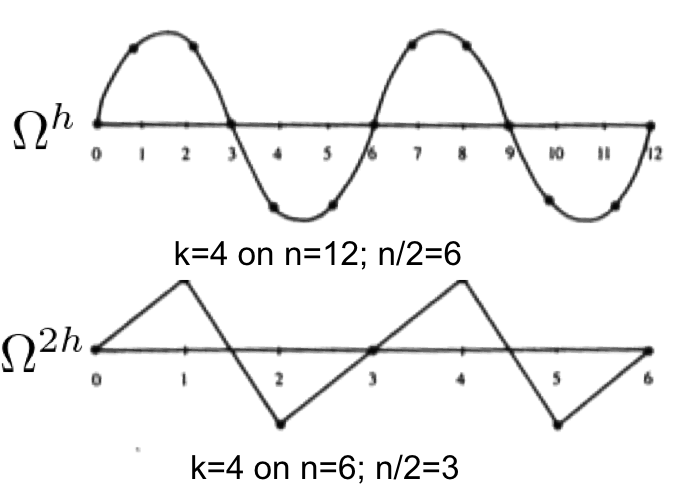
\includegraphics [width=0.55\textwidth, height=0.33\textheight] {fig/FourierGridError}
   \end{center}
   \caption{Relative Oscillation of a Fourier Mode Mapped Between Two Grids}% \cite{Briggs2000}}
   \label{fig:FourierGridError}
\end{figure}

Using this information, multigrid methods can be understood. The error is mapped from a fine grid to a coarser grid. A smoother is applied on the coarse grid to remove the newly oscillatory error components. The result is mapped back to the fine grid and used to correct the solution there. A few more relaxations are done back on the fine grid. That whole process is called a v-cycle. %, which is described in Algorithm~\ref{algo:MG}. 
A call to this method is symbolized as $v^h \leftarrow \ve{G}(v^h, b^h)$ and is effectively doing $v^{h} \approx \ve{G}^{-1}b^{h}$. A v-cycle algorithm is shown here:
%
\begin{list}{}{}
    \item Relax $\nu_1$ times on $\ve{A}^h u^h = b^h$ on the fine grid $\Omega^h$ using initial guess $v^h$.
    \item Compute the residual $r^h = b^h - \ve{A} v^h$. 
    \item Using some restriction operator, $\ve{R}_h^{2h}$, restrict the residual to a coarser grid: $r^{2h} =  \ve{R}_h^{2h} r^h$. 
    \item Solve the residual equation $\ve{A}^{2h} e^{2h} = r^{2h}$ on the coarse grid $\Omega^{2h}$. 
    \item Using some prolongation operator, $\ve{P}_{2h}^h$, prolong (interpolate) the coarse grid error back to a finer grid: $e^h = \ve{P}_{2h}^h e^{2h}$. 
    \item Add the error to the fine grid guess: $v^h \leftarrow v^h + e^h$. 
    \item Relax $\nu_2$ times on $\ve{A}^h u^h = b^h$ on $\Omega^h$ to get an improved solution. 
\end{list}

%The details of how restriction and prolongation are done are problem dependent. Simple iterative schemes can have very simple operators while more complex schemes may require more complex mappings. Other implementation choices are what relaxer to use and how many relaxations to do on each grid.
%
There are many variations of how multigrid methods are put together. All methods, however, are built on the basic v-cycle correction scheme. A V-cycle is an extension of the v-cycle. Instead of only using two grids, many grids are used. The problem is restricted from grid to grid until it is on some grid which is coarse enough to directly invert the equations. Then the errors are prolonged back up the chain, continuously correcting on finer grids, until the finest grid is reached. Multigrid methods are differentiated by how many times the V-cycle is done and how many grids are used. %A five-grid V-cycle can be seen in Figure~\ref{fig:Vcycle} (a). A W-cycle is when V-cycles are repeated to further improve the answer. An example can be seen in Figure~\ref{fig:Vcycle} (b). 
%\begin{figure}
%    \begin{center}
%      \includegraphics [width=0.7\textwidth, height=0.7\textheight, angle=180 ] {multigridFig}
%   \end{center}
%   \caption{Grid Schedule for (a) a V-cycle, (b) a W-cycle, and (c) a Full Multigrid Pattern \cite{Briggs2000}}
%   \label{fig:Vcycle}
%\end{figure}
%
%Multigrid can also be used to obtain an initial guess where much of the smooth error has been removed. This is called nested iteration, and the iterations begin on the coarsest grid and move up to the finest grid. If nested iteration is combined with V-cycles, the full multigrid method (FMG) is obtained, as seen in Figure~\ref{fig:Vcycle} (c). A call to any of the combinations of v-cycles is denoted $v \leftarrow \ve{G}(v, b)$. The optimal combination of grids and cycles may depend on problem type. The addition of more grids and cycles will reduce error, but at an added cost. 

Multigrid methods can be thought of as stationary iterative schemes that can be used alone or as accelerators for other methods. In the past these methods were highly problem specific and only applied to second-order elliptic PDEs. Over time they have been extended to different problem types, geometries, and discretizations.% \cite{Benzi2002}. 


%---------------------------------------------------------------------------------
\subsubsection*{Two Grid and Transport Two Grid}
The \textit{two-grid acceleration method} developed by Adams and Morel was one of the earlier spatial multigrid methods. %and it has been built upon by others \cite{Adams1993}. 
It is intended to accelerate convergence of the outer iterations for the transport equation when upscattering is present; the outer iteration method is Gauss Seidel and the method is only applied to upscattering groups. The original work was done for slab geometries with linear discontinuous (LD) discretization. %The general approach is expounded upon here to provide an example of multigrid methods applied to the transport equation and because a variation of this method is used in Denovo. 

Adams and Morel create a within group error equation by subtracting the GS equation from the transport equation. If the error in iteration $k$ is $\epsilon^k$ and the $l$th moment of the residual is $R_l^k$, then for group $g$ in 1-D this gives:
%
\begin{align}
   \mu \frac{\partial \epsilon_{g}^{k+1}(\mu)}{\partial x} + \Macro_{t,g} \epsilon_{g}^{k+1}(\mu) &= \sum_{l=0}^{L}\frac{2l+1}{4\pi} \bigl( \sum_{g'=1}^{G}\Macro_{s,g' \to g, l} \epsilon_{g',l}^{k+1} 
   +  R_{g,l}^{k+1}\bigr) P_{l}(\mu) \:,\label{eq:GSerror} \\
  \epsilon_{g}^{k+1}(\mu) &= \psi_{g}(\mu) - \psi_{g}^{k+1}(\mu) \:, \\
  \epsilon_{g',l}^{k+1} &= 2\pi \int_{-1}^{1}\epsilon_{g'}^{k+1}(\mu') P_{l}(\mu') d\mu' \:, \\ 
  R_{g,l}^{k+1} &=  \sum_{g'=g+1}^{G}\Macro_{s,g' \to g, l} \bigl( \phi_{g',l}^{k+1} - \phi_{g',l}^{k} \bigr) \:.
\end{align}
%
The diffusion approximation is applied to Equation \eqref{eq:GSerror}, giving a coarse grid equation (isotropic, one-group, diffusion equation). The fine grid is the \Sn equations for the upscattering groups.  

It is assumed that the zeroth moment of the error is a product of a spectral shape function, $\xi_g$, and a space-dependent modulation function, $E(x)$, giving
%
\begin{align}
  \epsilon_{g,0}^{k+1}(x) &= E(x)\xi_{g} \:, \text{ and} \label{eq:errorExpand} \\
  \sum_{g=1}^{G} \xi_{g} &= 1 \:.
\end{align} 
%
The spectral shape function corresponds to the slowest converging error mode, i.e.\ the mode to be eliminated. To find the shape function, Fourier analysis is performed on the GS iterative method. The zeroth moment of the cross sections is used to form the Fourier matrix, and then an eigenproblem can be formed. The spectral radius of the isotropic GS matrix is the eigenvalue, and the corresponding eigenvector is the shape function. Because the shape function is dependent on materials, one such calculation must be done for each material region. Note that by using the zeroth moment only the isotropic component of the solution is accelerated.

To restrict the residual, which is used as the source, to the coarse grid in the angular dimension, the anisotropic terms are truncated. To restrict to one energy group, the residual is simply summed in energy. The coarse grid equation is then solved on the coarse grid for the error. That error is prolonged to the fine grid and used to correct the flux there. The anisotropic terms are not recovered in the prolongation. The shape functions are used to expand the one group diffusion solution (error) into multiple groups. 

The coarse grid diffusion equations that result from Equations \eqref{eq:GSerror} and \eqref{eq:errorExpand} differ slightly in form from the standard diffusion equation in that there is an extra term containing the gradient of the shape function. This is zero in homogeneous regions, but undefined at material interfaces. Adams and Morel found that neglecting the gradient term all together still gave good results for their test problems. This may not be true for more complex cases.

The two-grid method requires the diffusion operator to be consistent with the transport operator, just like in DSA. This requirement can be difficult to meet for multi-dimensional problems, particularly for some spatial discretizations.% \cite{Adams1993}. 

The \textit{Transport two-grid (TTG) acceleration scheme} is based on the one developed by Adams and Morel. %As noted above, the iteration procedure uses a collapsed one-group diffusion equation to correct the low-order Fourier modes. %\cite{Adams1993}.
%Because of the consistency requirement for the discretization of the diffusion operator in multi-dimensional and multi-material problems, this method can fail for systems of interest.% \cite{Evans2009d}. 
%
The original two-grid method was modified by Evans et al.\ to make it applicable for multi-dimensional and multi-material problems by using a one-group transport equation instead of the diffusion equation. Adams and Morel showed that the slowest converging spatial modes are diffusive and can be exactly computed in the infinite homogeneous case. To preserve this, the TTG method gives the correct error estimation in that limit.% \cite{Evans2009d}. 

The cross sections used in TTG are therefore calculated to give the same energy-collapsed cross sections as the diffusion equation for the infinite homogeneous case, as seen in Equations \eqref{TTGxsecs1} and \eqref{TTGxsecs2}. TTG solves a one-group transport equation for the low-order error in each GS iteration, where $[g1, g2]$ is the group range of the upscatter block:
%
\begin{align}
  \ve{\hat{\Omega}} \cdot \nabla \psi_{\epsilon} &+ \bar{\Macro}\psi_{\epsilon} = \frac{1}{4\pi}\bar{\Macro}_{s}\phi_{\epsilon} + \frac{1}{4\pi}\bar{R} \:, \\
  \bar{\Macro} &= \frac{1}{\sum_{g=g_1}^{g_2} \frac{1}{\Macro^g}\zeta^g} \label{TTGxsecs1} \:,\\
  \bar{\Macro}_{s} &= \frac{1}{\sum_{g=g_1}^{g_2} \frac{1}{\Macro^g}\zeta^g} - \sum_{g=g_1}^{g_2} \bigl(\Macro^g\zeta^g - \sum_{g'=g_1}^{g_2} \Macro_{s0}^{gg'} \zeta^{g'} \bigr) \label{TTGxsecs2} \:. 
\end{align}
%
The spatial components of the error are $\psi_{\epsilon}$ and $\phi_{\epsilon}$; $\bar{R}$ is the residual. Just as in the original method, it is assumed that the error is separable in space and energy at each iteration: $\epsilon_g^k = \phi_g - \phi_g^k = \phi_{\epsilon}(\vec{r})\zeta^g$, where $\zeta^g$ is a material-dependent spectral function.% \cite{Evans2009d}. 

To execute the TTG scheme, a transport sweep in conducted in each group, a residual is calculated, the low-order transport solve described above is performed, an error form of the transport sweep is conducted, and the scalar flux is updated. All of that can be seen in the following equations: 
\begin{align}
  \ve{L}_g \psi_g^{k+\frac{1}{2}} &= \ve{M}\bigl(\ve{S}_{gg}\phi_g^{k+\frac{1}{2}} + \sum_{g'=g_1}^{g-1} \ve{S}_{gg'}\phi_{g'}^{k+\frac{1}{2}} + \sum_{g'=g+1}^{g_2}\ve{S}_{gg'}\phi_{g'}^k \bigr) + q_{e,g}  \:, \\
  R^{k+\frac{1}{2}}_g &= \ve{M} \sum_{g'=g+1}^{g_2}\ve{S}_{gg'} \bigl( \phi_{g'}^{k+\frac{1}{2}} - \phi_{g'}^k \bigr) \:, \qquad l = m = 0 \:, \\
  \bar{\ve{L}}\psi_{\epsilon} &= \ve{M\bar{S}} \phi_{\epsilon} + \bar{R} \:, \qquad l = m = 0 \:, \label{TTGerrorEqn} \\
  \phi_g^{k+1} &= \phi_{g}^{k+\frac{1}{2}} + \phi_{\epsilon}\zeta^g \:, \qquad l = m = 0 \:.
\end{align}
The operators with over-bars use the collapsed cross sections given in Equations \eqref{TTGxsecs1} and \eqref{TTGxsecs2}, and $\bar{R} = \sum_{g=g_1}^{g_2} R_g^{k+\frac{1}{2}}$. 

The $\zeta_g$ term is calculated from the eigenvalue problem obtained through Fourier analysis of the GS method using isotropic scattering, just like the original two-grid method:
%
\begin{equation}
  \bigl(\ve{\Sigma} - \ve{S}_L + \ve{S}_D\bigr)^{-1} \ve{S}_U\zeta = \rho\zeta \:,
\end{equation}
where $\ve{\Sigma}$ is the diagonal, total cross section matrix. As with the original two-grid method, the TTG method is limited to correcting only the isotropic flux moments. This is an adequate limitation as these moments are dominant in thermal groups where upscattering is most prevalent.%\cite{Evans2009d}.   

The additional cost of the method is like solving one extra group, so for cases with many upscattering groups the cost can be amortized. The acceleration equation can be preconditioned with DSA for additional speed. Finally, a reduced quadrature set can be used when solving Equation~\eqref{TTGerrorEqn} to limit the cost. Some test problems have shown TTG to be quite effective in improving the speed of convergence for upscatter problems when compared to unaccelerated GS.% \cite{Evans2009d}.




\end{document}
